\documentclass{article}

\usepackage{graphicx}
\usepackage{tikz}
\usepackage{tikzsymbols}
\usetikzlibrary{calc,patterns,shapes.geometric}
\pagestyle{empty}
\usepackage[margin=0pt]{geometry}
\geometry{papersize={14in,12in}}

\def\centerarc[#1](#2)(#3:#4:#5){\draw[#1] ($(#2)+({#5*cos(#3)},{#5*sin(#3)})$) arc (#3:#4:#5);}

\begin{document}
	\begin{figure}
		\centering
		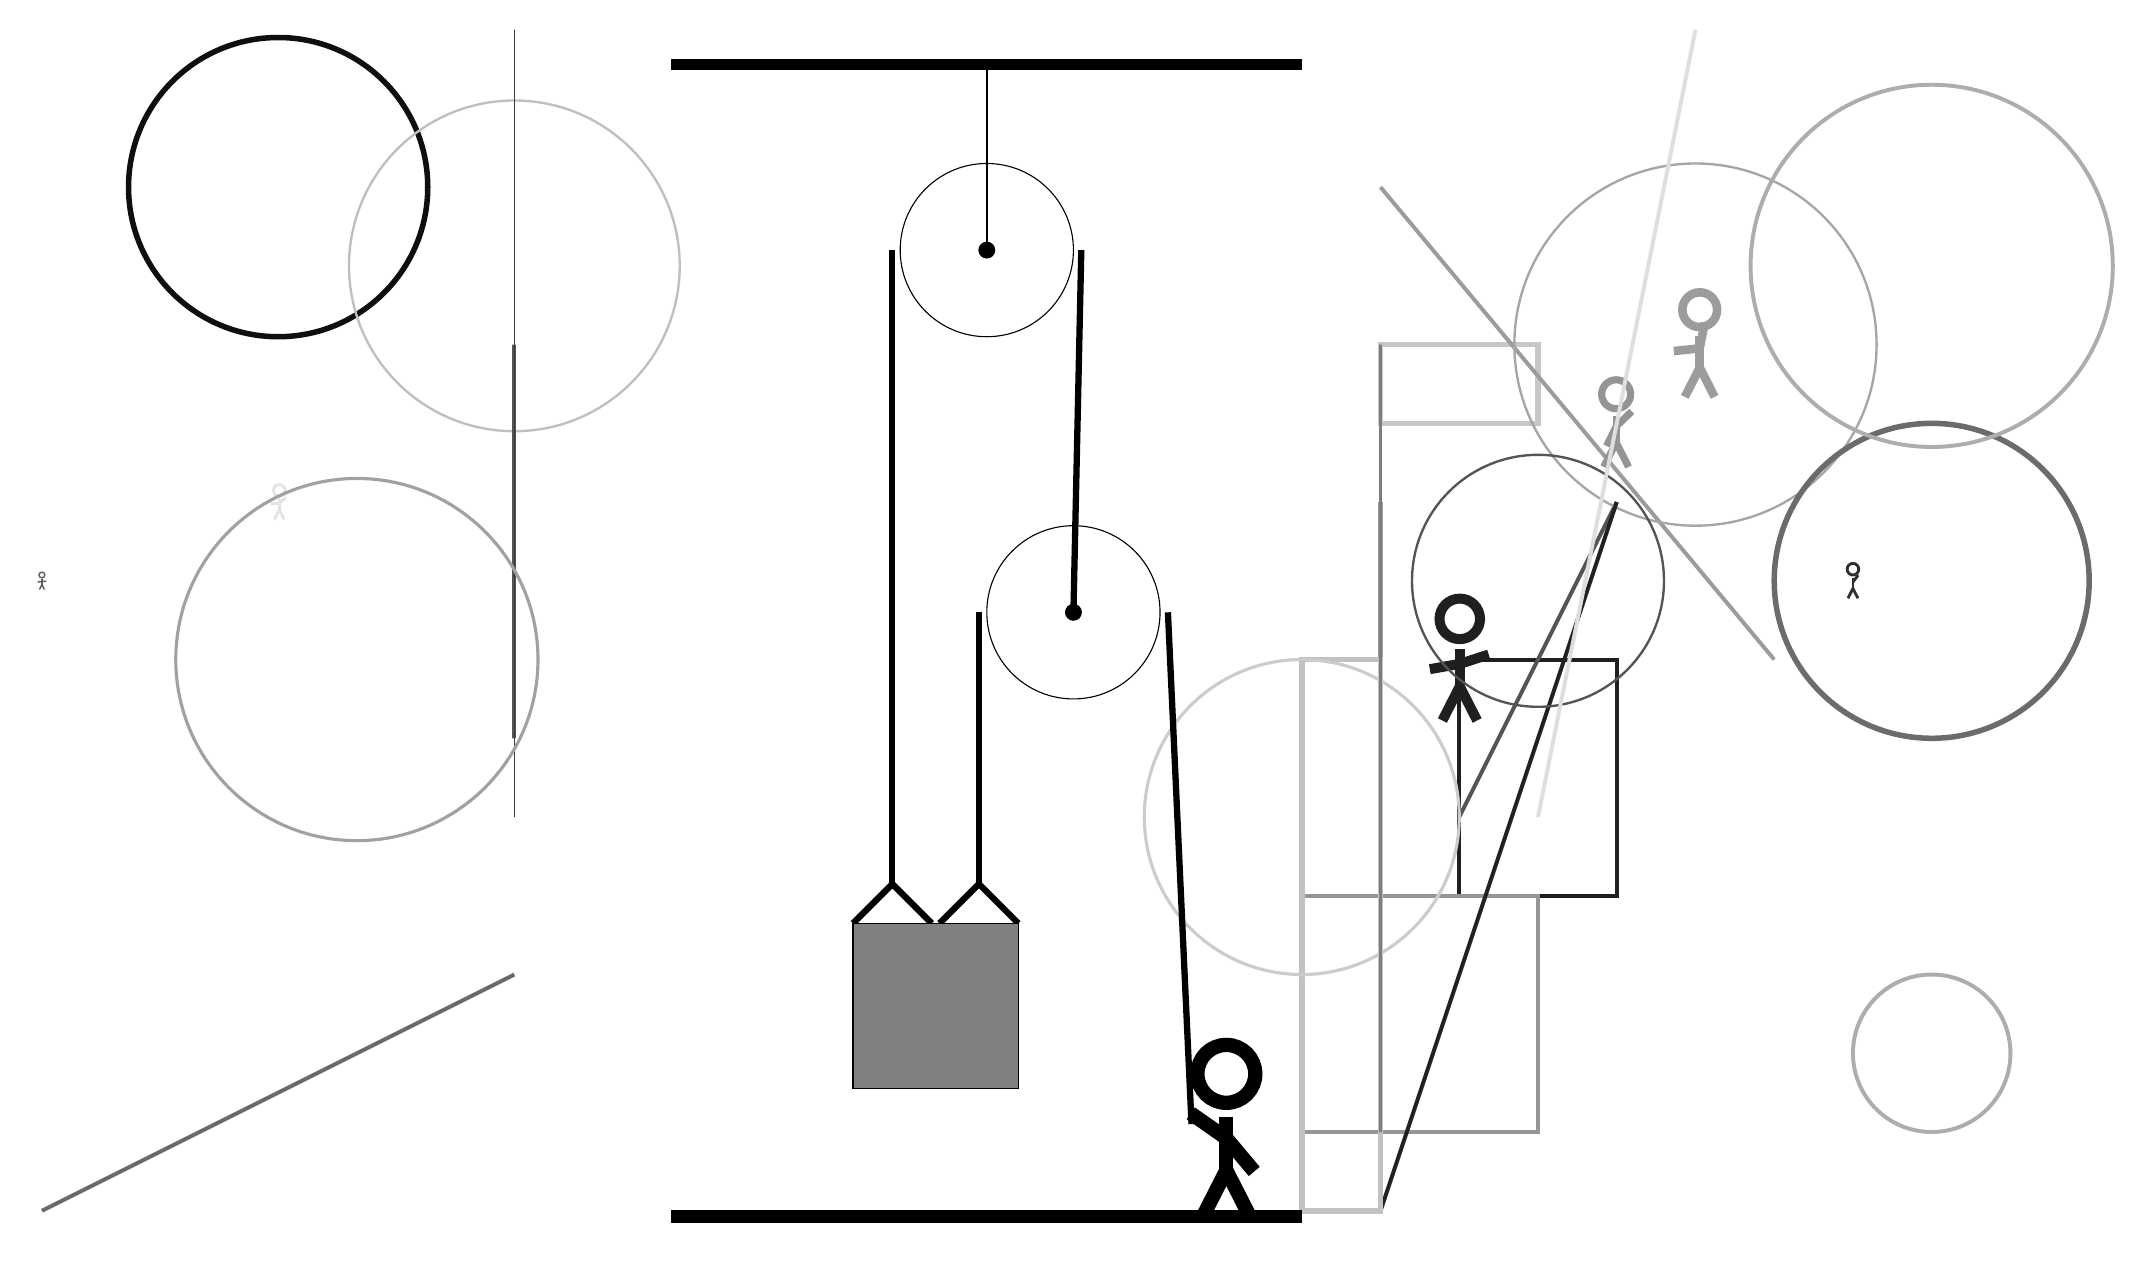
\begin{tikzpicture}
			%%%%% START %%%%%
			
			\draw[fill=black] (-2, 11.5) rectangle (6, 11.625);
			
			\draw (2, 9.2) circle (1.1);
			\draw[fill=black] (2, 9.2) circle (0.1);
			\draw[thick] (2, 9.2) -- (2, 11.5);
			
			\draw (3.1, 4.6) circle (1.1);
			\draw[fill=black] (3.1, 4.6) circle (0.1);
			
			\draw[line width=0.5mm, color=black!88] (8, 1) rectangle (10, 4);
			
			\draw[line width=0.7mm, color=black!22] (7, 7) rectangle (9, 8);
			\draw [line width=0.7mm, color=black!94](-7, 10) circle (1.9);
			\draw[line width=0.5mm, color=black!39](7, 10) -- (12, 4);
			\draw[line width=0.5mm, color=black!67](10, 6) -- (8, 2);
			
			\node[line width=0.3mm, color=black!42] at (10, 7) {\Strichmaxerl[5][64][44]};
			\node[line width=0.7mm, color=black!88] at (8, 4) {\Strichmaxerl[7][10][18]};
			\node[line width=0.2mm, color=black!63] at (-10, 5) {\Strichmaxerl[1][8][3]};
			\draw[line width=0.7mm, color=black!39] (7, -1) rectangle (7, 6);
			\draw[line width=0.5mm, color=black!41] (6, -2) rectangle (9, 1);
			
			\draw [line width=0.3mm, color=black!25](-4, 9) circle (2.1);
			\draw [line width=0.3mm, color=black!35](11, 8) circle (2.3);
			\draw [line width=0.5mm, color=black!32](14, -1) circle (1.0);
			
			\draw[line width=0.5mm, color=black!67] (-4, 3) rectangle (-4, 8);
			\draw[line width=0.2mm, color=black!77] (-4, 2) rectangle (-4, 12);
			\draw[line width=0.5mm, color=black!87](7, -3) -- (10, 6);
			\draw[line width=0.7mm, color=black!24] (7, -3) rectangle (6, 4);
			\node[line width=0.4mm, color=black!11] at (-7, 6) {\Strichmaxerl[2][3][42]};
			\draw [line width=0.4mm, color=black!37](-6, 4) circle (2.3);
			
			\draw[line width=0.2mm, color=black!69] (7, -1) rectangle (7, 8);
			\draw [line width=0.3mm, color=black!67](9, 5) circle (1.6);
			\draw[line width=0.5mm, color=black!13](9, 2) -- (11, 12);
			
			\draw [line width=0.4mm, color=black!20](6, 2) circle (2.0);
			\node[line width=0.5mm, color=black!81] at (13, 5) {\Strichmaxerl[2][90][53]};
			\draw [line width=0.7mm, color=black!58](14, 5) circle (2.0);
			\draw[line width=0.5mm, color=black!59](-4, 0) -- (-10, -3);
			
			\node[line width=0.3mm, color=black!39] at (11, 8) {\Strichmaxerl[6][6][79]};
			\draw[line width=0.3mm, color=black!51] (7, 8) rectangle (7, -2);
			
			\draw [line width=0.5mm, color=black!32](14, 9) circle (2.3);
			
			\draw[line width = 0.8mm]  (0.3, 0.65) -- (0.8, 1.15) -- (1.3, 0.65);
			\draw[line width = 0.8mm]  (1.4, 0.65) -- (1.9, 1.15) -- (2.4, 0.65);
			\draw[fill=black!50] (0.3, 0.65) rectangle (2.4, -1.45);
			
			\draw[line width = 0.8mm] (0.8, 9.2) -- (0.8, 1.15);
			\centerarc[line width = 0.8mm](2, 9.2)(0:180:1.2000000000000002);
			\draw[line width = 0.8mm] (3.2, 9.2) -- (3.1, 4.6);
			\draw[line width = 0.8mm] (1.9, 4.6) -- (1.9, 1.15);
			\centerarc[line width = 0.8mm](3.1, 4.6)(0:180:1.2000000000000002);
			\draw[line width = 0.8mm] (4.3, 4.6) -- (4.6, -1.9);
			
			\node at (5, -2) {\Strichmaxerl[10][-35][-50]};
			
			\draw[fill=black] (-2, -3) rectangle (6, -3.15);
			
			%%%%% END %%%%%
		\end{tikzpicture}
	\end{figure}	
\end{document}